\section{AMIDST model class}\label{section:AMIDSTmodelClass}

One of the main goals of AMIDST project is the definition of a general model class with the following characteristics: 

\begin{itemize}
\item \textbf{Feature 1:} it should be applicable to the three considered use-cases, i.e., Daimler, Cajamar, and Verdande,

\item \textbf{Feature 2:}  it should be general enough to be applicable to any future, potentially similar, use-cases and

\item \textbf{Feature 3:} it should be scalable, supporting both inference and learning from massive data streams.

\end{itemize}

Taking these different characteristics into account and using the subnetwork graphical notation introduced in Section \ref{SubSection:GraphicalNotation}, the general AMIDST model class, as well as its specific instantiation to each use case, are first introduced and discussed in Section \ref{GeneralModelClass}. A summary is finally included in Section \ref{summaryAMIDSTModels}.

%-----------------------------------------------------------------------------------------------------------------------------------------
\subsection{The general AMIDST model class}\label{GeneralModelClass}
%-----------------------------------------------------------------------------------------------------------------------------------------

Figure \ref{Figure:AMIDSTModelClass} shows the proposed general AMIDST model class. This model is the result of combining all the models that have been previously defined for the different use cases. As it can be seen, subnetworks have been used to group variables with similar properties, so that the commonalities between all models are taken into account. 

\begin{figure}[ht!]
\begin{center}
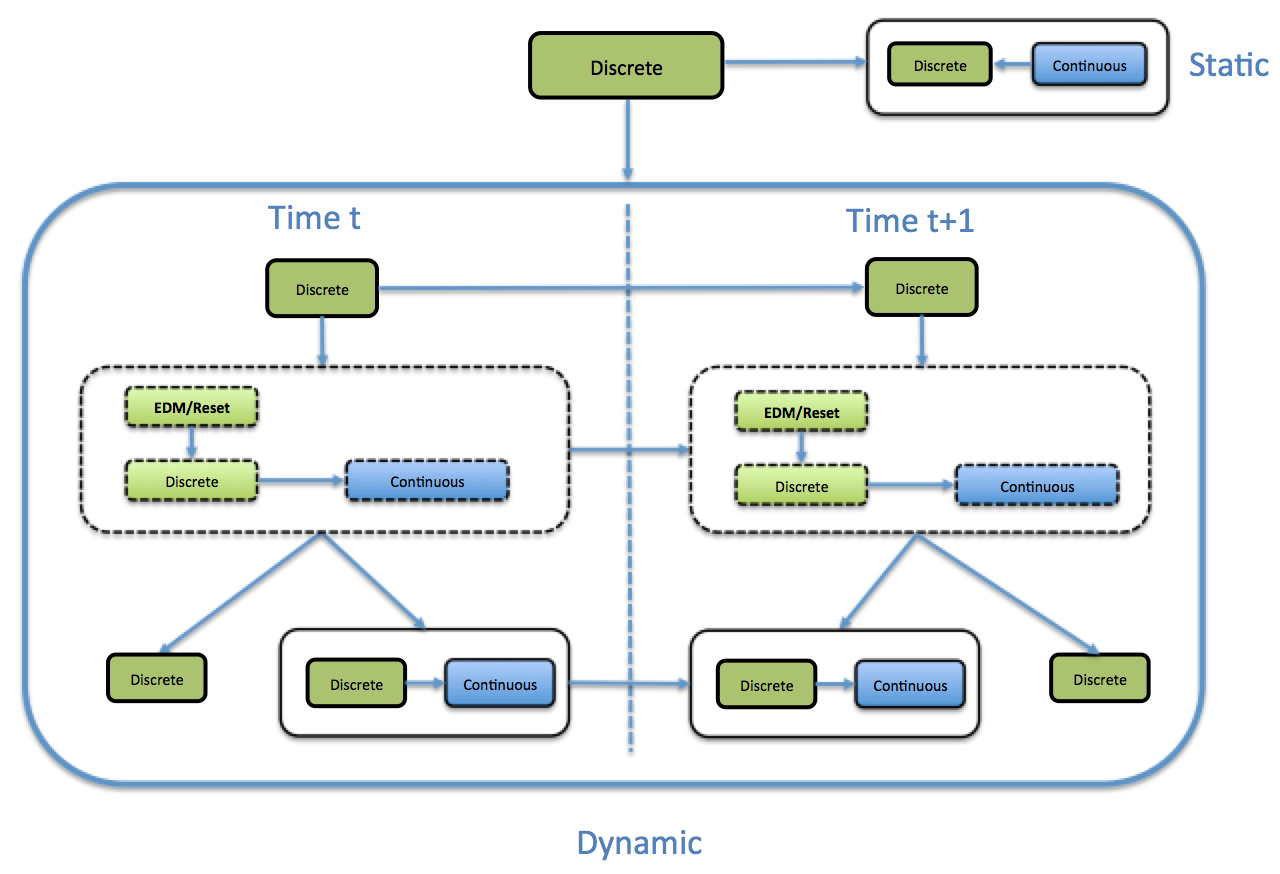
\includegraphics[scale=0.465]{./figures/AMIDSTModelClass}
\caption{\label{Figure:AMIDSTModelClass} General AMIDST model class.}
\end{center}
\end{figure}

The general AMIDST model class can be seen as a 2T-DBN (see Section \ref{SubSubSection:2DBNs}), i.e., it satisfies the first order Markov property and the stationary assumption. However, this model is not as general as a 2T-DBN and presents a more restricted internal structure that offers a good trade-off between expressiveness and efficiency. More precisely, the structure of this model decomposes along three main different layers which can be described, at time $t$, as follows:

\begin{itemize}

\item \textbf{Control/class layer:} The upper layer corresponds to a subnetwork including either continuous or discrete observed variables, that can act for instance as either control continuous variables or a class variable respectively. These set of variables can be connected through consecutive time steps to encode temporal dependences, e.g., the probability of a particular class label at time $t+1$ varies with respect to its label at time $t$. 

The links from the continuous observed variables to the state subnetworks in the \textit{Hidden layer} (i.e., the set of State 1 and State 2 variables) will be possibly handled with logit and probit functions.

\item \textbf{Hidden layer:}  The middle layer corresponds to a set of interconnected discrete and continuous hidden subnetworks, for which only links from discrete to continuous subnetworks are allowed. We will use the term \textit{state} variables to refer to the set of discrete hidden variables in both State 1 and State 2 subnetworks, and the term \textit{latent}\footnote{The term \textit{latent} for variables is generally used in statistics to refer to hidden variables as opposed to observed ones. However, we will use it here to exclusively refer to continuous hidden variables.} variables to refer to the set of continuous hidden variables in the Latent subnetwork.

This layer can contain state variables that are not connected over time, and that could be used, for instance, to model mixture of Gaussian distributions over the observed continuous variables in the \textit{Observable layer}. Moreover, state and latent variables that are connected over time can be used to model a process that is evolving and changing over time. Recall that, links from latent variables to state variables are strictly prohibited.

\item \textbf{Observable layer:} The bottom layer corresponds to a subnetwork including both discrete and continuous observed variables. These variables can in principle be interconnected but, in our different use cases, only links from discrete to continuous nodes are required. However, in general, there is no restriction on the direction of the links between the variables in this layer. In addition, it is possible to alleviate the sensor Markov assumption by including links between observed variables at consecutive time steps.

\end{itemize} 

This model class can also be parametrized in alternative ways to improve the expressibility and applicability to different problems or domains. In general, this model class falls inside the conditional linear Gaussian framework, so the conditional probability distributions are parameterized as detailed in Section \ref{SubSection:HybridBNs}. But this model class might also contain instantiations which are not covered by this general framework. More precisely, when the top layer class is instantiated to  a continuous subnetwork then the conditional probabilities of ``State 1'' and ``State 2'' will be instantiated with logistic or probit distributions, because we have continuous parents with discrete children. Additionally, we also envision the possibility of introducing in the observable layer the use of probability distributions belonging to the MoTBF family \cite{Langseth12} to extend the modelling capacities of this model class.

In the following sections, we will show how this model class satisfies the aforementioned \textbf{Feature 1}, by describing how each particular use case fits in this restricted 2T-DBN AMIDST model. This instantiation process of the general AMIDST model to the three use-cases (all of them with different application scenarios) can also be seen as a practical example demonstrating the general applicability of the resulting AMIDST model class. This hence gives arguments in favour of \textbf{Feature 2} and shows how the AMIDST model class can be potentially instantiated to other future use cases. Finally, the remaining task is related to \textbf{Feature 3} and consists of designing inference and learning algorithms that allow the application of the AMIDST model to massive data streams. 



%-----------------------------------------------------------------------------------------------------------------------------------------
\subsubsection{Daimler model class}\label{daimlerAMIDSTModels}
%-----------------------------------------------------------------------------------------------------------------------------------------

Daimler's model class has been previously displayed in Figure \ref{Figure:daimlerLEdynGeneric}. Taking the general AMIDST model class into account, Daimler's model class can be reinterpreted, according to Figure \ref{Figure:AMIDSTModelClassDaimler}, as follows:

\begin{figure}[ht!]
\begin{center}
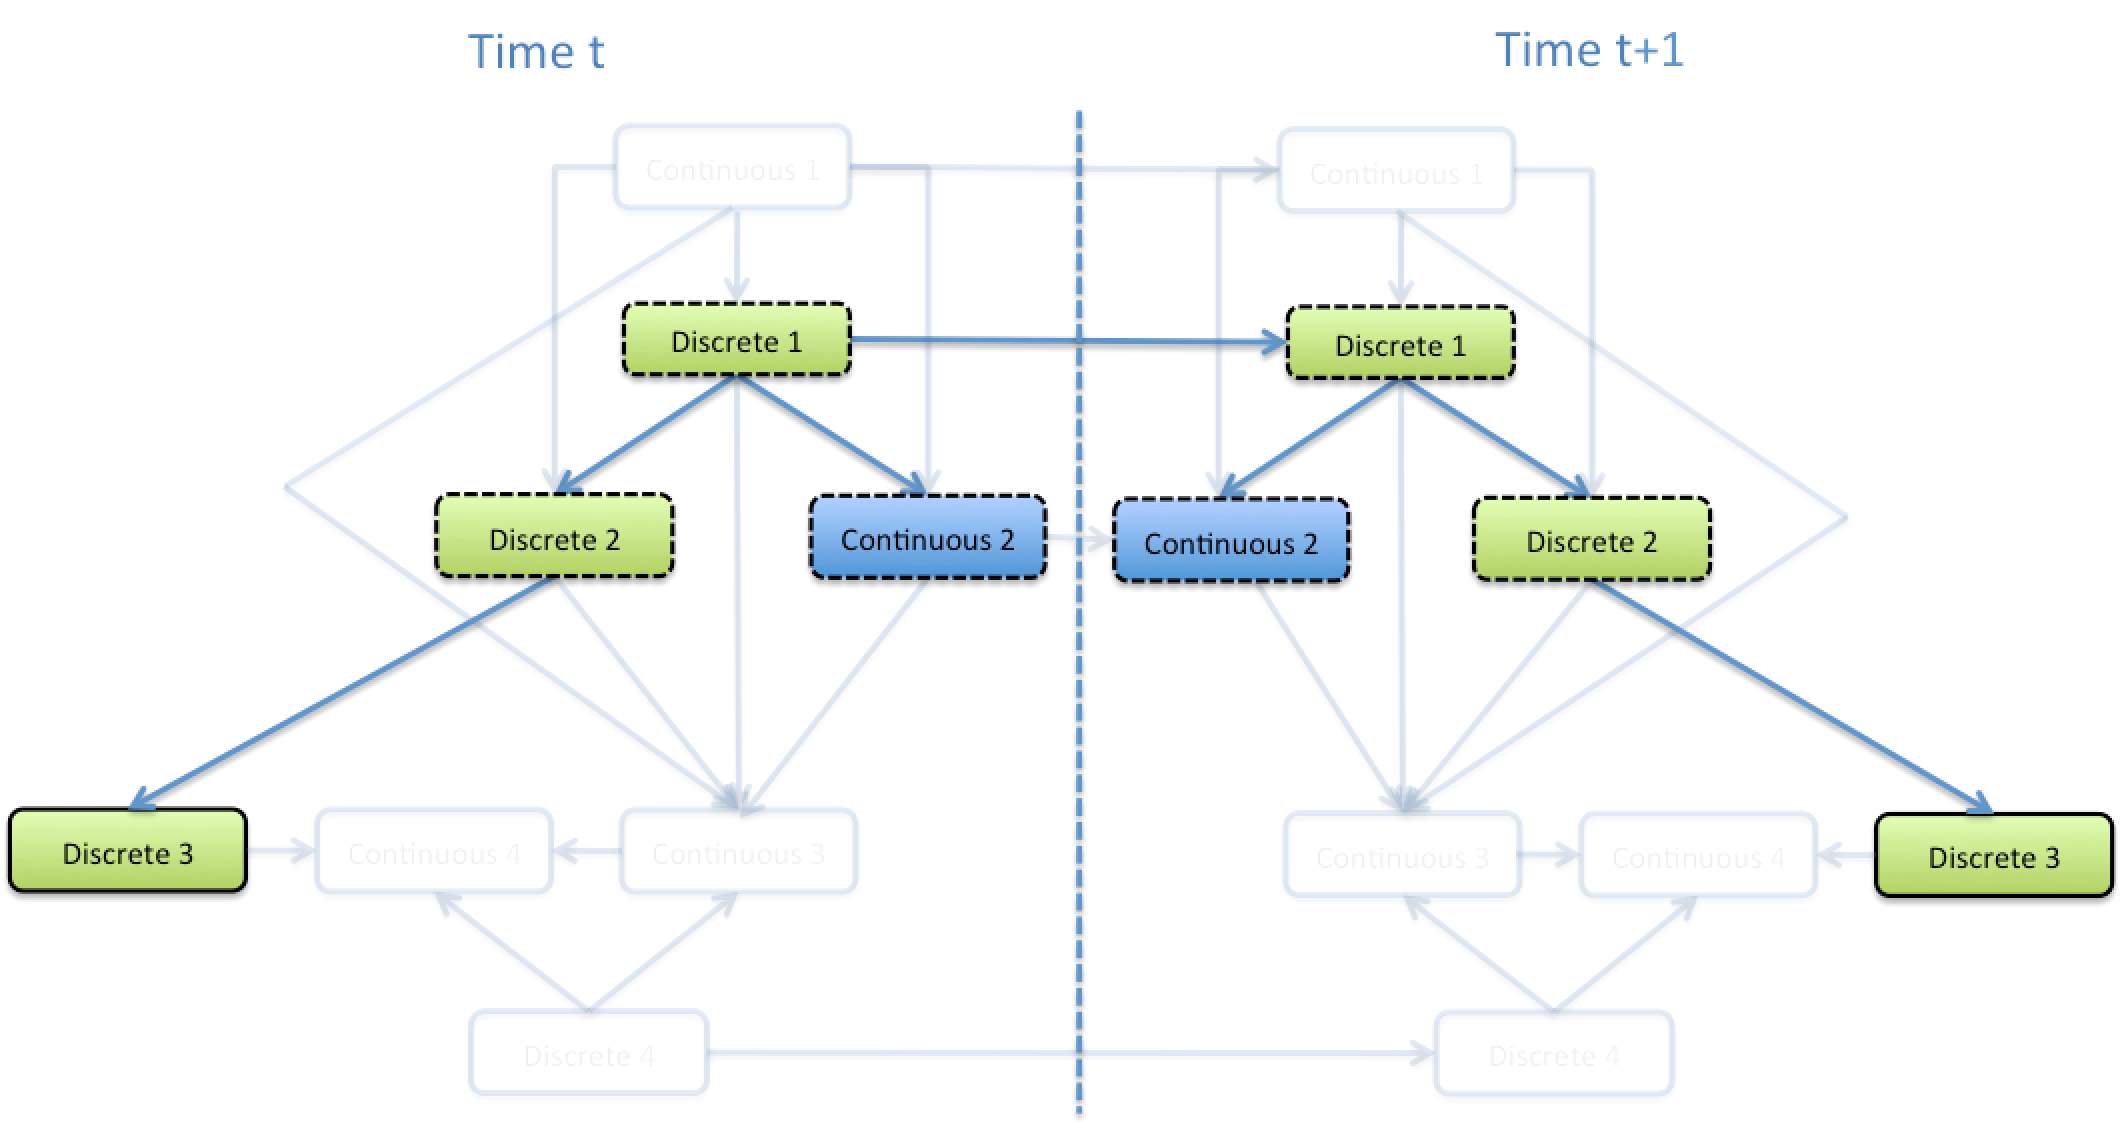
\includegraphics[scale=0.39]{./figures/AMIDSTModelClassDaimler}
\caption{\label{Figure:AMIDSTModelClassDaimler} AMIDST model class - Daimler}
\end{center}
\end{figure}

\begin{itemize}

\item \textbf{Control/class layer}: is not used in this domain.

\item \textbf{Hidden layer}: the two sets of state variables are required here. 

The lower set of state variables (i.e., State 2 subnetwork in Figure \ref{Figure:AMIDSTModelClass}) encode a polytree \cite{JensenNielsen2007} for the hierarchy of Hypothesis. This polytree structure, not explicitly encoded in the model, can indeed be exploited during inference.

Connection through time is only made at the top level state variables (i.e., State 1 subnetwork in Figure \ref{Figure:AMIDSTModelClass}), which correspond to the signal real values (S\_REAL\footnote{Although these variables are inherently continuous, we notice that they are discretized to avoid the inference problems derived of having continuous parents with discrete children (see Section \ref{Section:DaimlerDynamic}).}). Consequently, the future and past time slices of our 2T-DBN are conditionally independent given S\_REAL variables corresponding to the present time. 

In addition, inside a time slice, the observed continuous and hidden discrete subnetworks are also conditionally independent given S\_REAL variables. In the case that we want to contemplate a possible extension in which the lower level Hypothesis are connected over time, then State 1 subnetwork would contain both the S\_REAL variables and the temporally linked Hypothesis. However, as commented before, this would greatly complicate the inference process. 

\item \textbf{Observable layer:} there are two sets of observed variables in this case. On one hand, we encounter a group of variables representing the measured data (S\_MEAS), along with the variables encoding the sensor noise (S\_SIGMA). The resulting structure is again a polytree, which presents some advantages for the inference process. On the other hand, we have a single discrete node for the manoeuvre Event, which will be the target variable during inference. 

\end{itemize}

%-----------------------------------------------------------------------------------------------------------------------------------------
\subsubsection{Cajamar model class}\label{cajamarAMIDSTModels}
%-----------------------------------------------------------------------------------------------------------------------------------------

Concerning Cajamar use-case, both application scenarios share the same models with two possible versions, namely, static and dynamic (see Section \ref{Section:CajaMarModels}). At this point, we obviate the static version, because the general AMIDST model class is primarily a dynamic model class. Therefore, the high-level description of Cajamar's dynamic model (previously displayed in Figure \ref{fig:component}) can be reinterpreted according  to Figure \ref{Figure:AMIDSTModelClassCajamar}. 

\begin{figure}[ht!]
\begin{center}
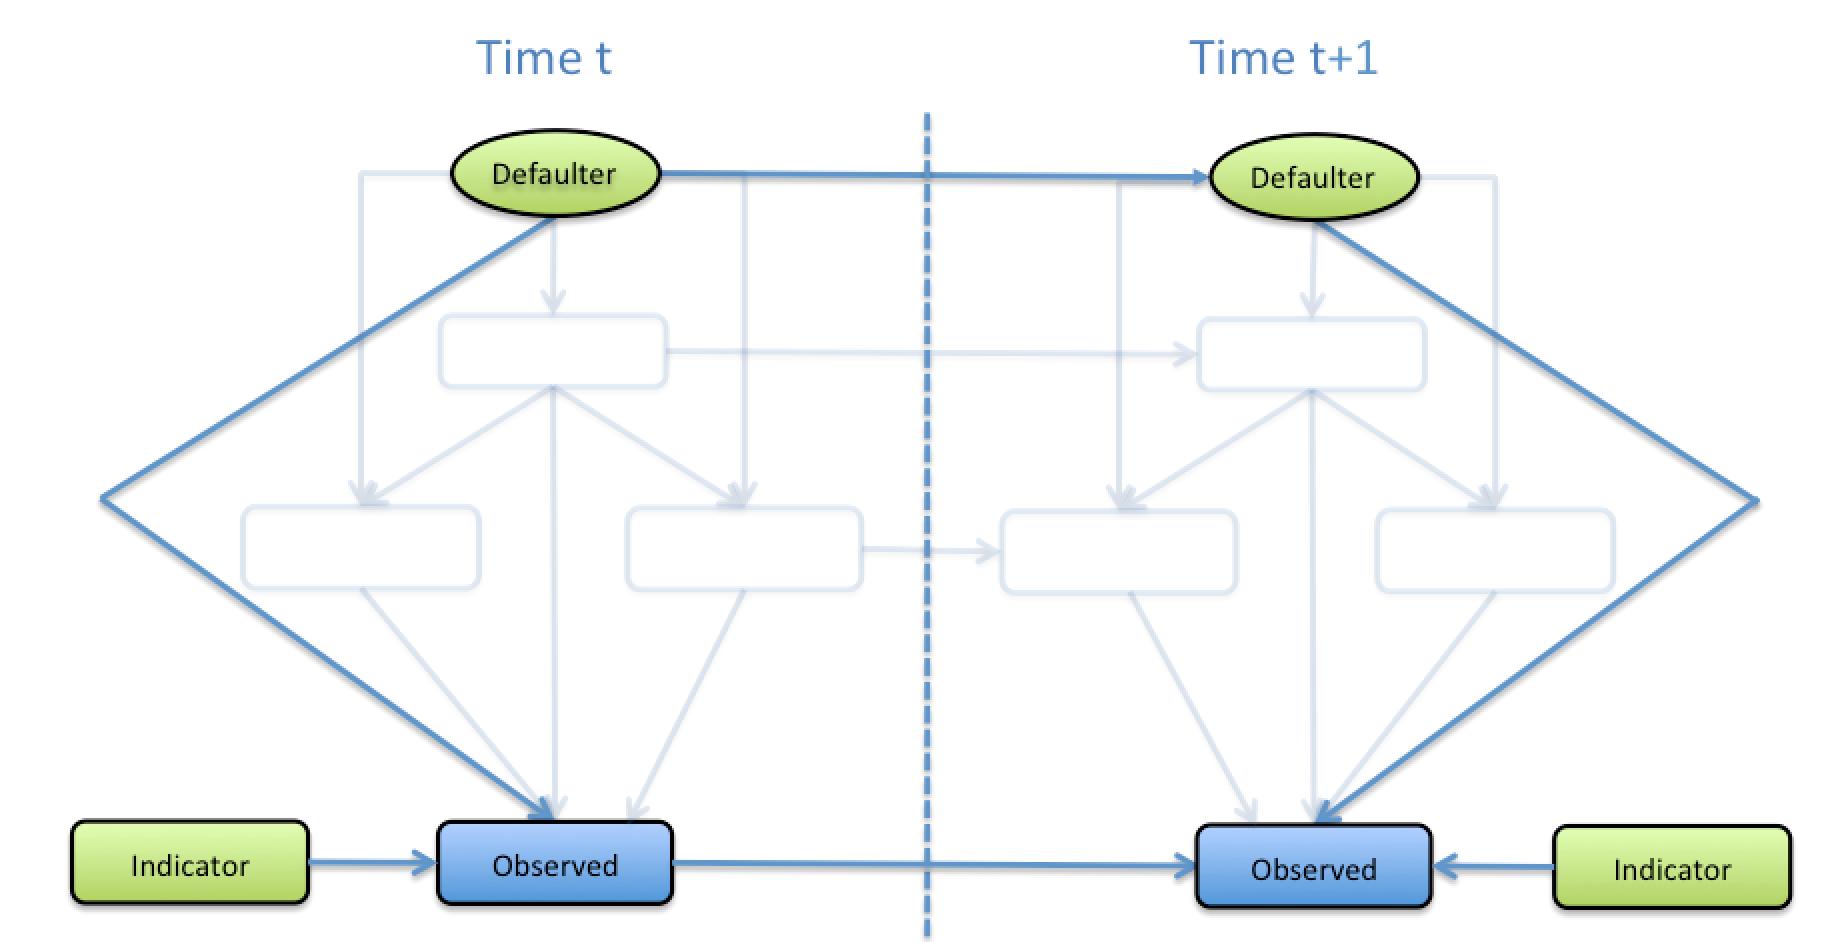
\includegraphics[scale=0.39]{./figures/AMIDSTModelClassCajamar.png}
\caption{\label{Figure:AMIDSTModelClassCajamar} AMIDST model class - Cajamar.}
\end{center}
\end{figure}


Following the layer-wise analysis used above, Cajamar's model is described as follows:
\begin{itemize}

\item \textbf{Control/class layer}: the top node ``Defaulter" in this layer represents the class variable to categorize a client as defaulter or non-defaulter. There exist temporal links between consecutive time steps to model the dynamic nature of being a defaulter or non-defaulter. Note that this is indeed the target variable in the inference process.

\item \textbf{Hidden layer}: is not used in this domain.

\item \textbf{Observable layer:} The ``Observed" continuous subnetwork represents information corresponding to the socio-demographic variables, memory variables, financial activity, and past payment behaviour of a client, which, in principle, may or may not be connected over time. Moreover, the ``Indicator" discrete subnetwork includes the set of indicator discrete variables denoted as $\delta_{X_t}$. These indicator variables are used for modelling situations where some variables in the ``Observed" continuous subnetwork have a large number of zeros.

\end{itemize}



%---------------------------------------------------------------------
\subsubsection{Verdande model class}\label{verdandeAMIDSTModels}
%---------------------------------------------------------------------

Figure \ref{Figure:AMIDSTModelClassVerdande} shows how the general AMIDST model class is instantiated in the case of Verdande. This instantiated model encompasses the models of the three applications scenarios detailed in Figures \ref{Figure:VTScenario1}, \ref{Figure:VTScenario2} and \ref{Figure:VTScenario3}  (see Section \ref{Section:VerdandeModels}).  We now comment the main elements of this instantiated model.


\begin{itemize}
\item \textbf{Control/class layer}:  This element is instantiated to a set of nodes modelling the observed control variables. In the three application scenarios, the role of this control variables is to condition the transition probability of the state variables and allow the modelling of non-stationary transition probabilities.  

\item \textbf{Hidden layer}: This element is directly instantiated from the general class. However, there are some differences when applied to each particular application scenario. For the first application scenario (see Figure \ref{Figure:VTScenario1}),  ``State 2'' is not needed and ``State 1'' is instantiated to the ``Normal/Abnormal'' state variable. For the second application scenario, ``State 1'' is no needed and ``State 2'' is instantiated to a single multinomial variable whose role is to model mixture of Gaussians at the leaves. In the third application scenario, ``State 2'' is no used and ``State 1'' is instantiated to a sub-network containing the FormationDetection and Switch nodes. 

\item \textbf{Observable layer: } This element of the model class is similarly instantiated in the three application scenarios. In the case of application scenario 1 and 3, it is just instantiated to a single response variable. In the application scenario 2, this instantiation can be made over a set of (possibly interconnected) response variables. 
\end{itemize}



\begin{figure}[ht!]
\begin{center}
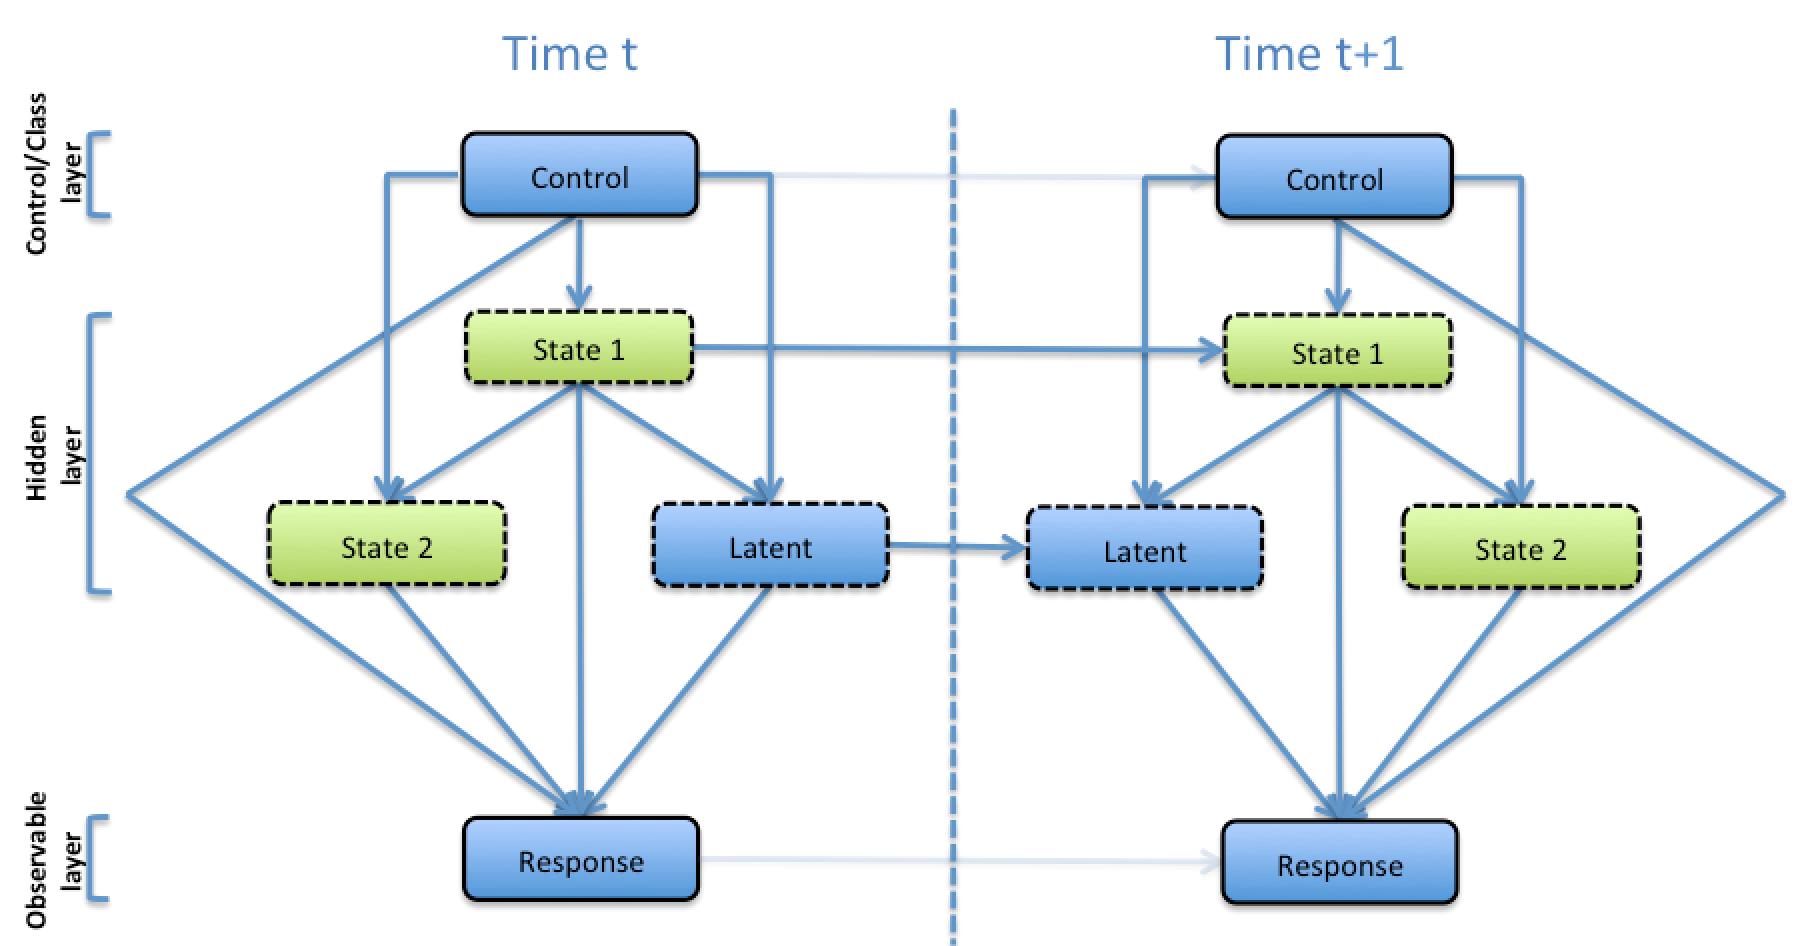
\includegraphics[scale=0.39]{./figures/AMIDSTModelClassVerdande}
\caption{\label{Figure:AMIDSTModelClassVerdande} AMIDST model class - Verdande.}
\end{center}
\end{figure}


\subsection{Summary}\label{summaryAMIDSTModels}

As it has been shown in the previous sections, the proposed AMIDST model class of Figure \ref{Figure:AMIDSTModelClass} encompasses the different application scenarios of the three use cases. These three use-cases come from very different domains: automotive, finance and oil-drilling. In our opinion, these are strong arguments in favour of the generality and applicability of this model class. Although, in any case, a better understanding of the faced problems and/or future applications might reveal that some elements of this model class need to be refined.  

A higher level view of our proposed AMIDST model is displayed in Figure \ref{Figure:AMIDSTModelClassHighLevel}. As commented before, it shows how the AMIDST model class could actually be seen as a ``restricted" 2T-DBN. It is restricted in three different ways. Firstly, all the nodes are structured in three layers, each one with clear semantics while modelling: Broadly speaking, the \textit{control/class layer} represent control variables that may affect the process homogeneity/stationarity, or represent the class variable in classification tasks; the \textit{hidden layer} includes a sufficiently rich set of hidden variables to capture the process dynamics; and the \textit{observable layer} encompasses sensor measures and predictive attributes. The second restriction states that, in opposite to general 2T-DBNs, the variables in this model class can only be temporally linked to other variables in the same layer. And, finally, the last restriction  states that continuous hidden variables cannot point to discrete (hidden or observed) nodes. This last constraint implies that our inference algorithms will not have to deal with the hard and open problem of computing posterior distributions or marginalize over continuous variables which are parents of discrete children nodes. So, in most of the cases, the network can be parameterized using the conditional linear Gaussian framework. And in those cases when this is not possible, because the instantiated model contains continuous parents with discrete children, we will have that the continuous nodes are always observed. 

\begin{figure}[ht!]
\begin{center}
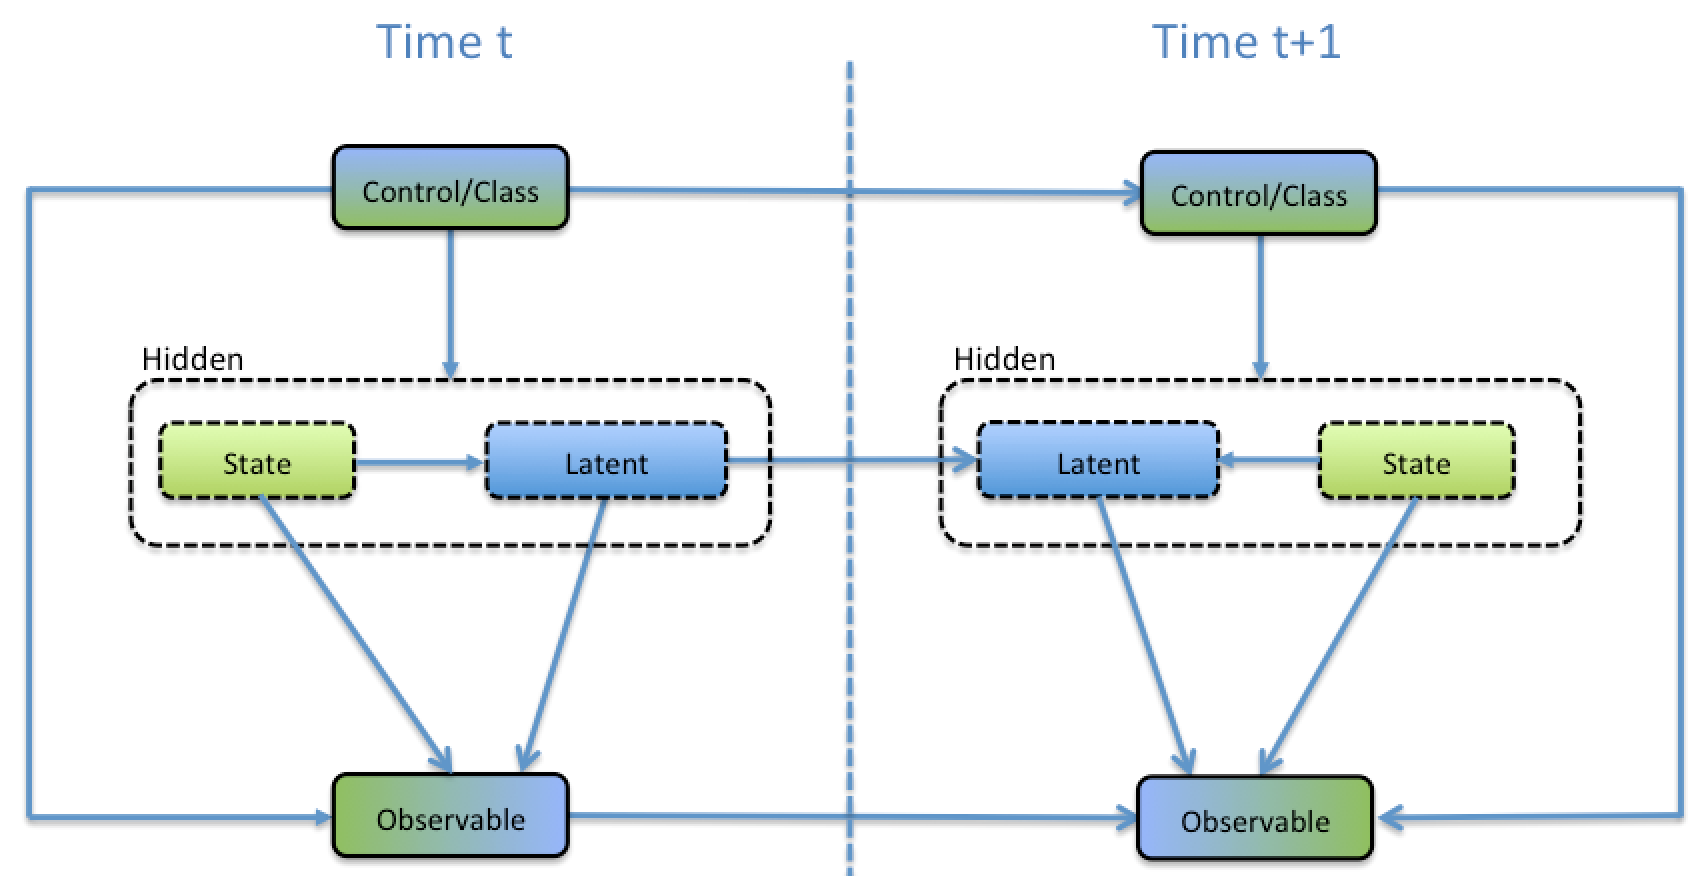
\includegraphics[scale=0.4]{./figures/AMIDSTModelClassGeneral}
\caption{\label{Figure:AMIDSTModelClassHighLevel} The high-level AMIDST model class}
\end{center}
\end{figure}


%This section, with the high-level figure, should help to defend the third point made in the introduction, i.e., that it should be general enough to be applicable to any future, potentially similar, use-cases.
 


%\begin{figure}[ht!]
%\begin{center}
%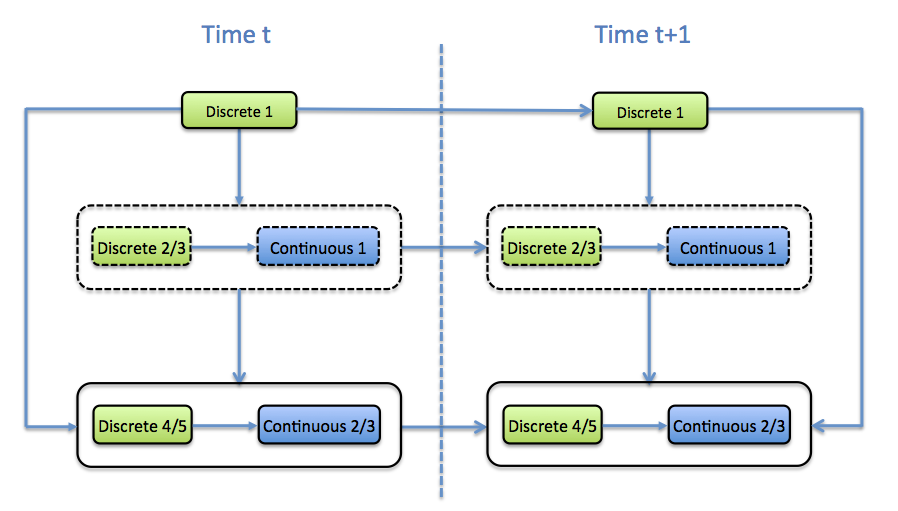
\includegraphics[scale=0.4]{./figures/AMIDSTModelClassHighLevel}
%\caption{\label{Figure:AMIDSTModelClassHighLevel} AMIDST model class high level}
%\end{center}
%\end{figure}

%\begin{figure}[ht!]
%\begin{center}
%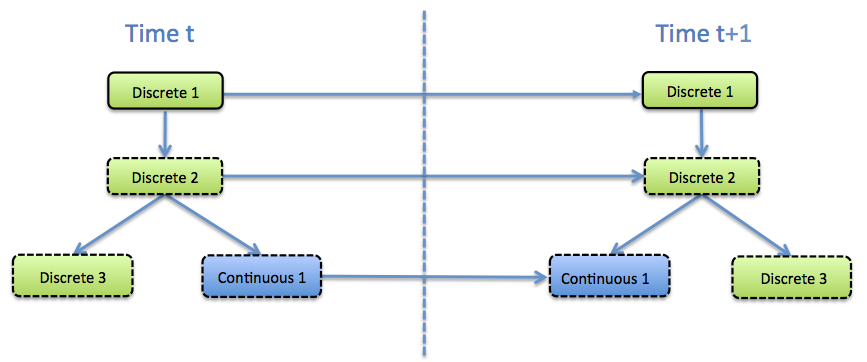
\includegraphics[scale=0.4]{./figures/AMIDSTModelClassTopPart}
%\caption{\label{Figure:AMIDSTModelClassHighLevel} AMIDST model class top part}
%\end{center}
%\end{figure}
%
%\begin{figure}[ht!]
%\begin{center}
%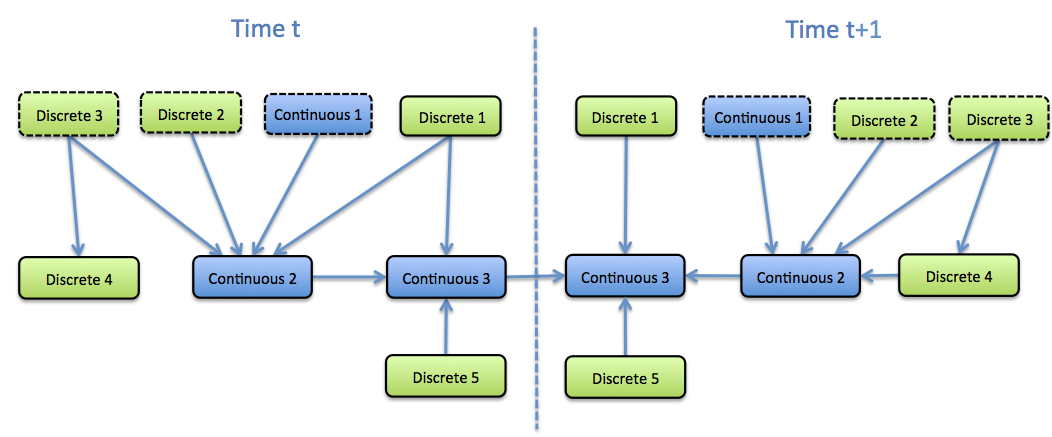
\includegraphics[scale=0.4]{./figures/AMIDSTModelClassLowPart}
%\caption{\label{Figure:AMIDSTModelClassHighLevel} AMIDST model class low part}
%\end{center}
%\end{figure}